\section{Limits on \mueee from Muon Decays}
In section \ref{sec:mu3e_experiment}, we saw how the production rate of $\mu^+$ at \mueee could be brought to the level of muon decays occuring at a rate $\order(10^9) \mu^+/s$.
The signal for the \mueee experiment, $\mu^+ \rightarrow e^+ e^+ e^-$, contains no missing energy as there are no neutrinos in the final state.
The SM has many avenues to produce such a signal with missing energy through muon decay, and we will go through the relevant backgrounds to our limits here.
Since the experiment is looking at a muon beam, it can be expected that there will be many events that behave like a muon decay and have missing energy.
Our signal will overlap with the backgrounds present and \mueee, and will allow us to study the signal component of $\mu^+ \rightarrow e^+ \bar{\nu}_\mu \nu_e e^+ e^-$.

For this experiment, we have utilized \madgraph to do the final state integration, as our signal will have four particles in the final state, and this is difficult to do by hand.
Furthermore, even though we will be looking at a four body decay, the scalar particle will be on-shell and decay later to an $e^+ e^-$ pair, and \madgraph will also take care of generating the events corresponding to this decay.
All of the diagrams that \madgraph generates are available in appendix \ref{app:muon_diagrams}.

\subsection{Backgrounds}
Here we will discuss the relevant backgrounds to the experiment and their initial implications on their effects on our limits.

A strong irreducible background for the experiment is

\begin{equation}
    \mu^+ \rightarrow e^+ + \bar{\nu}_\mu + \nu_e + e^+ + e^-
\end{equation}

\noindent which comes with a branching ratio of $3.4 \times 10^{-5}$ \cite{Agashe:2014kda}. 
This is due to an internal conversion of muon to electron with a weak vertex, just like an ordinary muon decay, also known as a Michel decay.
To remove this background process, momentum conservation can be applied provided that the energy resolution is small enough.
For \mueee, a total energy resolution of $\sigma_E < 1\textrm{MeV}$ is sufficient for sensitivity of branching ratios down to $10^{-15}$ \cite{Blondel:2013ia}.
One such diagram for this process is shown in Fig.\ \ref{fig:mu_eeenunu_SM}.

\begin{figure}[h]
    \centering
    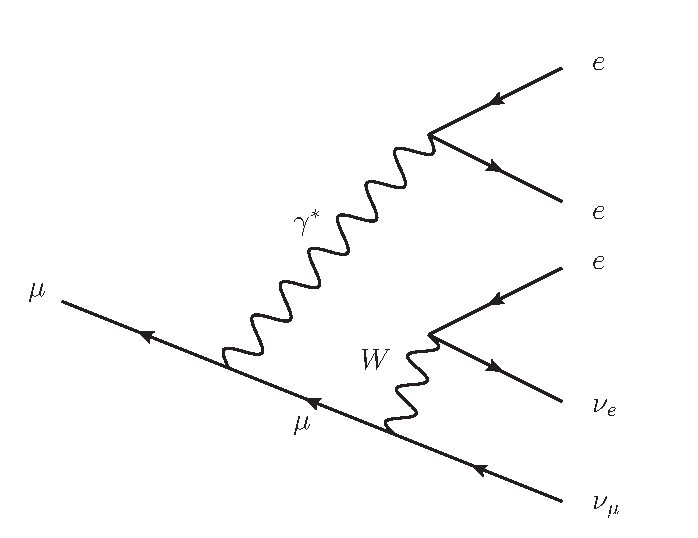
\includegraphics[width = 0.6\textwidth]{Figures/feynman_diagrams/mu_eeenunu_SM.eps}
    \caption{One Feynman diagram for the process $\mu^+ \rightarrow e^+ \bar{\nu}_\mu \nu_e e^+ e^-$. Here a virtual photon is emitted and decays to an $e^+ e^-$ pair. Note that the photon can be radiated off of any of the charged particles in the diagram before the $e^+ e^-$ decay. This background process can be suppressed by using momentum conservation with a high energy resolution.}
    \label{fig:mu_eeenunu_SM}
\end{figure}


Another source of background for the experiment is the radiative muon decay

\begin{equation}
    \mu^+ \rightarrow e^+ + \bar{\nu}_\mu + \nu_e + \gamma
\end{equation}

\noindent where the $\gamma$ radiates off of either the muon or electron.
This process comes with a branching ratio of $1.4 \times 10^{-2}$, given a photon energy larger than $10\textrm{MeV}$ \cite{Agashe:2014kda}.
The photon can then convert to an $e^+ e^-$ pair in the detector or target material, and mimic the irreducible background above.
Conversions outside of the target can be supressed if the vertex can be readily identified.
Within the target, this background appears as an accidental background with a regular muon decay.

There are other sources of background present as well.
We've already briefly mentioned Michel decays, which can be identified by the lack of any negatively charged particle tracks, since the experiment uses a $\mu^+$ beam.
Bhabha scattering from the positrons coming from either the muon decay, or a contaminated beam, scattering off of the target material make an $e^+ e^-$ pair appear from a single vertex.
This has missing energy from the unaccounted electron in the target material, and can be removed as the irreducible background.
Finally, there are also pions that may contaminate the beam and decay either to $\pi^+ \rightarrow e^+ e^+ e^- \nu_e$, or $\pi^+ \rightarrow \mu^+ \nu_\mu \gamma$ with the photon converting to an $e^+ e^-$ pair, which have branching ratios $3.2 \times 10^{-9}$ and $2.00 \times 10^{-4}$ relatively \cite{Agashe:2014kda}.
It is expected that the pion contamination is on the order of $10^{-12}$ for the HiMB~\cite{Blondel:2013ia}, and the small decay rates should also suppress these numbers of events to safely negligible rates.

\subsection{Signal}
